% !TeX root = ../main.tex
% This section introduces the various embedded platforms that are available on the 5th semester.


\section{Embedded platform}
The goal of the 5th semester of the bachelor in Software is to develop an embedded system, making it is relevant to look into the different relevant platforms.
The university supplies the student groups with a LEGO Mindstorms base set, consisting of both a LEGO Mindstorms NXT 2.0 kit and a LEGO Mindstorms EV3 kit, as well as an assortment of sensors, motors and LEGO bricks.
In addition, other platforms can be ordered, and a few of the alternative options will be examined.

\subsection{LEGO Mindstorms}
LEGO Mindstorms is a programmable computer kit made by the LEGO Group.
The platform is based around a central control computer, called the Intelligent Brick, and includes a variety of sensors, motors and connection cables.

The LEGO Mindstorms platform comes with a graphical drag and drop interface for programming.
However, different compilers for a variety of programming languages exist as an alternative to the interface and as such, the choice between the different Mindstorms platforms, does not depend on language preferences.

\paragraph{LEGO Mindstorms NXT 2.0}
The LEGO Mindstorms NXT 2.0 (NXT), as shown on \autoref{fig:legonxt}, is the second generation LEGO Mindstorms kit.
The NXT Intelligent Brick is a micro computer based on the 32-bit 48 MHz ARM7 microprocessor with 256 kilobytes of flash memory and 64 kilobytes of RAM \cite{nxt2userguide} \cite{nxt2ev3compare}.
It includes a variety of sensors, such as touch, sound, light and distance sensors, as well as servo motors and lamps.

A potential major disadvantage of the NXT 2.0 is its age.
The platform was released in 2006, meaning that the software might have compatibility issues with modern operating systems.

\begin{figure}[!tbp]
	\centering
	\subfloat[The NXT 2.0 \cite{nxt2ev3compare}.]{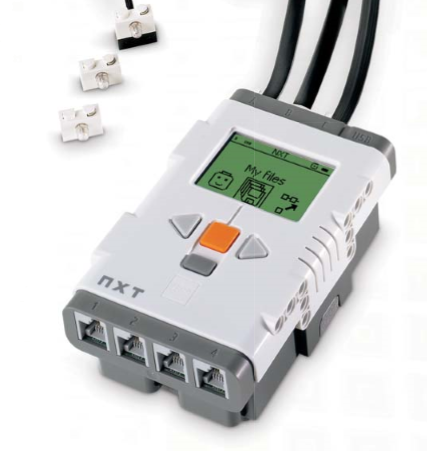
\includegraphics[width=0.4\textwidth]{images/legonxt}\label{fig:legonxt}}
	\hfill
	\subfloat[The EV3 \cite{ev3userguide}]{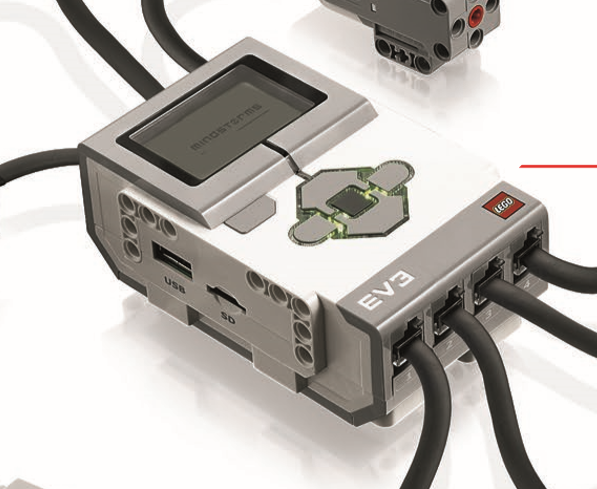
\includegraphics[width=0.4\textwidth]{images/legoev3}\label{fig:legoev3}}
	\caption{The LEGO Mindstorms.}
  \end{figure}

\paragraph{LEGO Mindstorms EV3}
The  LEGO Mindstorms EV3 (EV3), as shown on \autoref{fig:legoev3}, is the third generation of the LEGO Mindstorms series.
The EV3 mainly improves on the specifications of the second generation, adding a significantly more powerful 300MHz ARM9 processor, running Linux, 16 megabytes of flash memory, which is extendable with a microSDHC card and 64 megabytes of RAM \cite{ev3userguide}.
Furthermore, it adds remote control, WiFi capabilities, and more recently updated compilers and is fully backwards-compatible with the NXT sensors\cite{ev3nxtcompatability}.

Both are more akin to general purpose computers, designed for small electronics projects and both platforms include different models, with some being more powerful than others or having different features that further set them apart.


\subsubsection{Arduino}
The Arduino is a single-board computer platform as shown on \autoref{fig:arduinouno}, designed for small electronics projects by being easy to use from a hardware and software perspective.
The Arduino Corporation developed a language, APL, which is a subset of \texttt{C++}, which is most often used when working with the platform.
The primary advantage of the platform is that it is easy to work with and that there are so many different boards, all of which differ in performance, meaning that one that matches the particular requirements of the project most likely exists.
The IO possibilities of the Arduino are General Purpose Input Output (GPIO) pins, which can connect to most types of sensors and motors, as these are, as implied by the name, general purpose.
The Arduino-ecosystem is comprised of different boards, all of which are built for different purposes.
Differences being in processing power, as well as pins.
The Arduino Uno is most commonly used board in the ecosystem \cite{ArduinoUno3}, and has a 12 MHz ATmega328P processor and 2 kilobytes of RAM.
A larger version, the Arduino Due has an 84 MHz processor and 96 kilobytes of RAM \cite{ArduinoDue}, and more input/output pins and is meant for larger scale Arduino projects.

\begin{figure}[!tbp]
	\centering
	\subfloat[Arduino Uno \cite{ArduinoUno3}.]{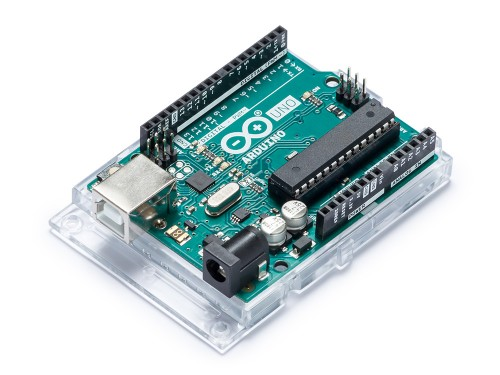
\includegraphics[width=0.4\textwidth]{images/arduino}\label{fig:arduinouno}}
	\hfill
	\subfloat[Raspberry Pi 3 B+ \cite{raspberrypi}]{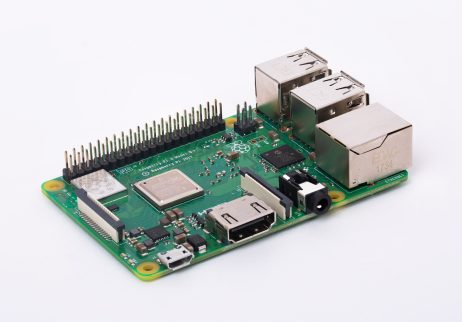
\includegraphics[width=0.4\textwidth]{images/raspberrypi}\label{fig:raspberrypi}}
	\caption{Single-board computers}
  \end{figure}

\subsubsection{Raspberry Pi}\label{subsec:rpispecs}
The Raspberry Pi, as shown on \autoref{fig:raspberrypi}, is a single-board computer eco-system which, like the Arduino, consists of small computers with GPIO pins.
It differs from the Arduino by having a full operating system, and generally being more powerful.
Additionally, the majority of the Raspberry Pi computers have more processing power and memory, and the newer versions include a Wi-Fi module.
They also come with a larger variety of ports - both USB, HDMI and jack, adding more possibilities for connectivity.

The newest version, Raspberry Pi 3 B+, features a 1.4 GHz quad-core CPU, with 1 gigabyte of RAM \cite{raspberrypi}.
They released a light-weight version, called the Raspberry Pi Zero, which trades performance, having only a 1 GHz single-core CPU and 512 megabytes of RAM, for a smaller footprint, being less power consuming, and a lower cost.

\subsection{Takeaways}
\label{platformtakeaways}
There are multiple platforms on which to build an embedded system.
This data is summed up in the following table.

\begin{table}[h]
	\begin{adjustbox}{max width=\textwidth}
	\begin{tabular}{|l|l|l|l|l|}
		\hline
		                & Processor                          & MHz 	& RAM in MB    & Flash Memory          	\\\hline
		NXT 2.0 		& 32-bit Atmel AT91SAM7S256 ARM7     & 48  	& 0.0625   & 256 KB                   	\\
		EV3     		& 32-bit TI Sitara AM1808 ARM9       & 300 	& 64   & 16 MB and microSDHC 			\\
		Arduino Uno    	& 8-bit AVR ATmega328                & 20  	& 0.00195    & 32 KB                    \\
		Arduino Due    	& 32-bit Atmel SAM3X8E               & 84  	& 0.09375   & 512 KB                   	\\
		Pi 3 B+      	& 64/32 bit ARM Cortex-A53 quad core & 1400 & 1024    & MicroSD slot            	\\
		Pi Zero       	& 32bit ARM1176ZF single core        & 1000 & 512  & MicroSD slot 					\\\hline
	\end{tabular}
\end{adjustbox}
\end{table}

The Raspberry Pi system can be quite powerful a project regarding embedded systems, which can also be said about the EV3.
This can be a disadvantage, as it does not allow full control of the execution order.
This issue will be analyzed in detail when looking into real-time systems.

The Arduino and NXT both have less processing power than the Raspberry Pi and EV3, and thus making them more interesting choices, by limiting the hardware capabilities.
The disadvantage of the Arduino is that it has fewer supported programming languages, and the fact that the GPIO ports make for hardware-related challenges, which is not the purpose of this semester.
Unlike the Arduino, the NXT offers easy to use hardware ports, and large variety of sensors and motors.
As the NXT is supplied by the university it is the obvious choice, especially considering the points provided in this section.

